%%%%%%%%%%%%%%%%%%%%%%%%%%%%%%%%%%%%%%%%%%%%%%%%%%%%%%%%%%%%%%%%%%%%%%%%%%%%%

\chapter{La sonate op. 27}

\begin{figure}[!p]
  \begin{bigcenter}
    \begin{tabular}{lr}
      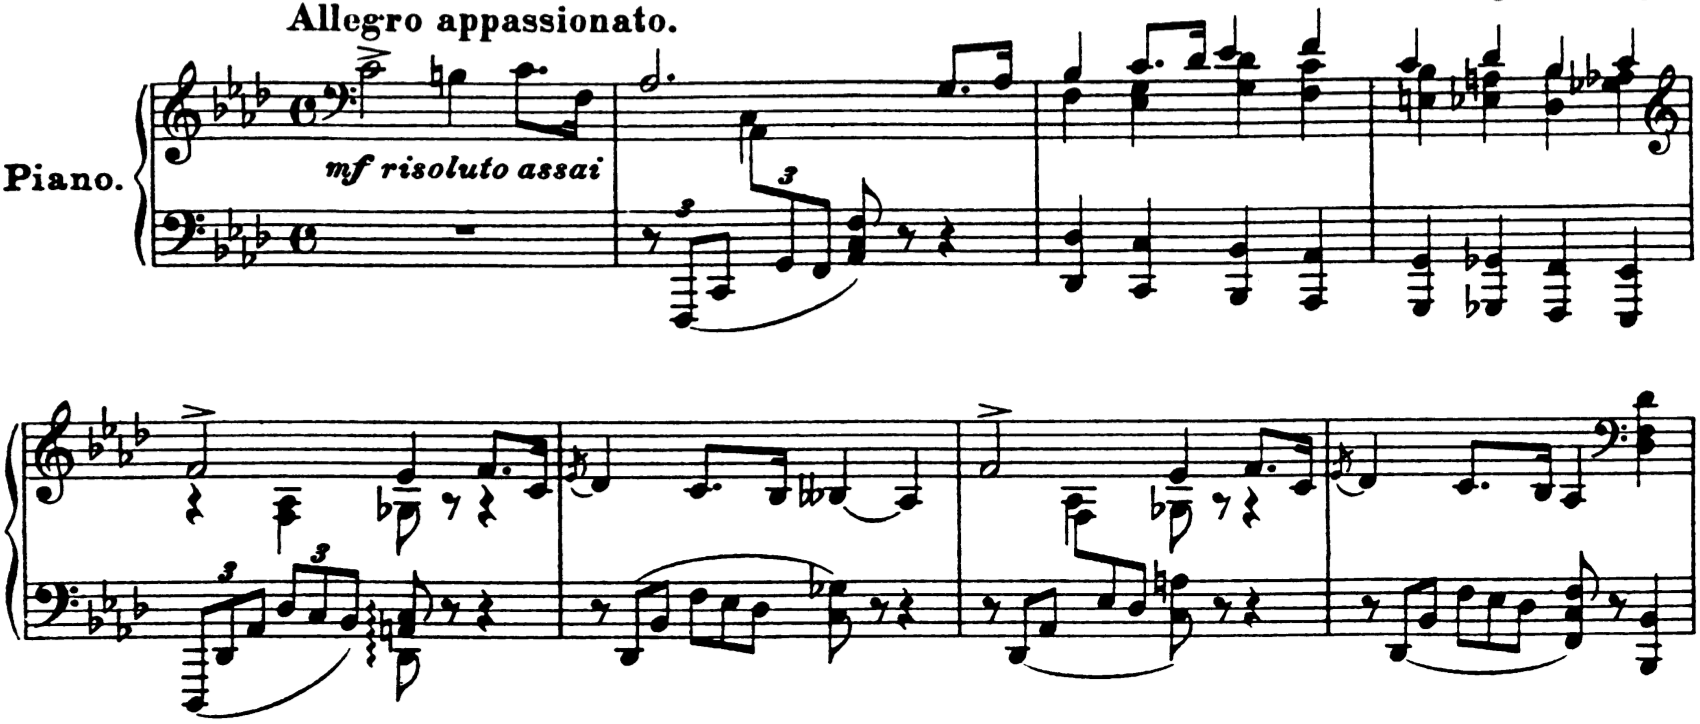
\includegraphics[width=12.5cm, keepaspectratio]{sonate-theme-1.png}
      &
      
\includegraphics[width=3cm, keepaspectratio]{op1-qr.png}
    \end{tabular}
  \end{bigcenter}
  \caption{\label{sonate-theme-1}Sonate en fa m Op.25, thème \no 1.}
\end{figure}

\begin{figure}[!p]
  \begin{bigcenter}
    \begin{tabular}{lr}
      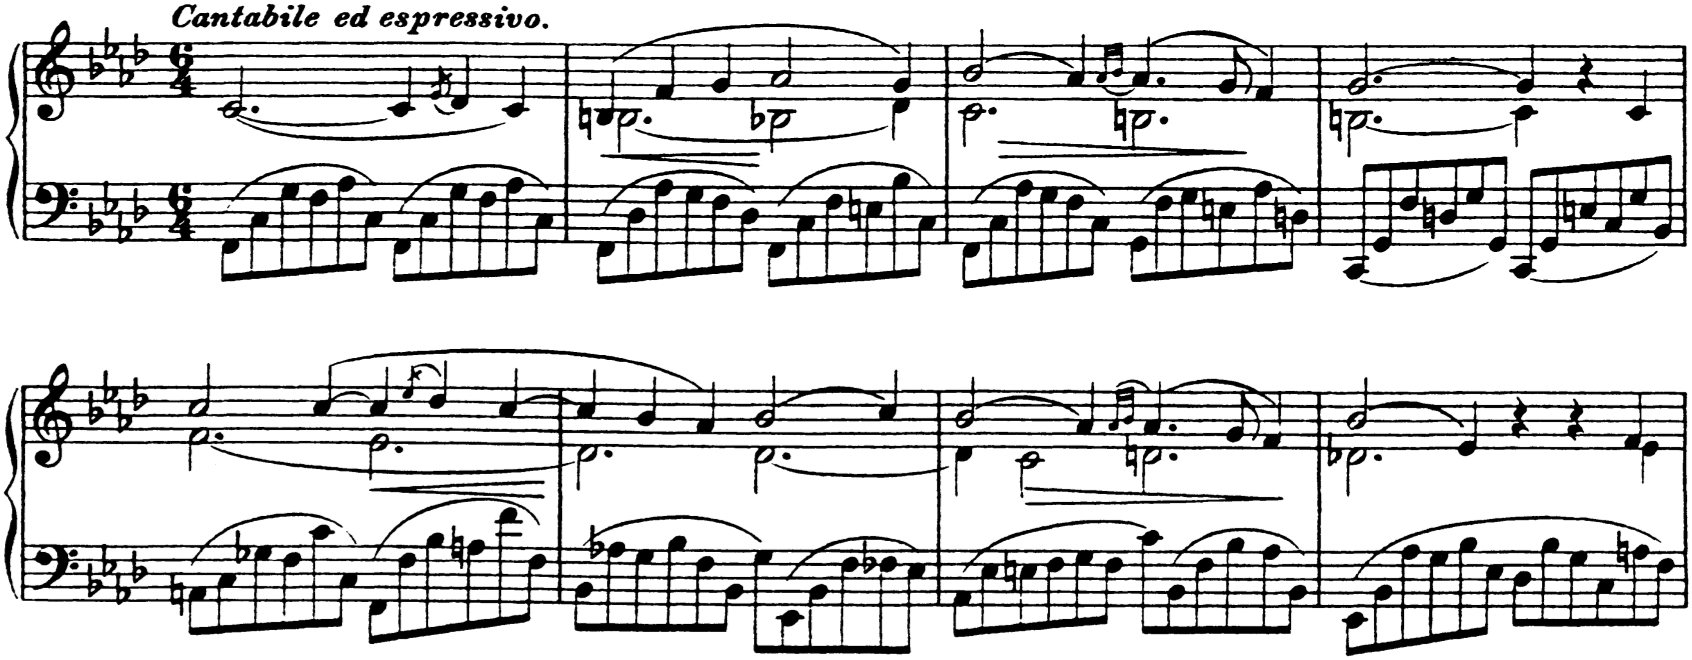
\includegraphics[width=12.5cm, keepaspectratio]{sonate-theme-2.png}
      &
      
\includegraphics[width=3cm, keepaspectratio]{op1-qr.png}
    \end{tabular}
  \end{bigcenter}
  \caption{\label{sonate-theme-1}Sonate en fa m Op.25, thème \no 2.}
\end{figure}

\begin{figure}[!p]
  \begin{bigcenter}
    \begin{tabular}{lr}
      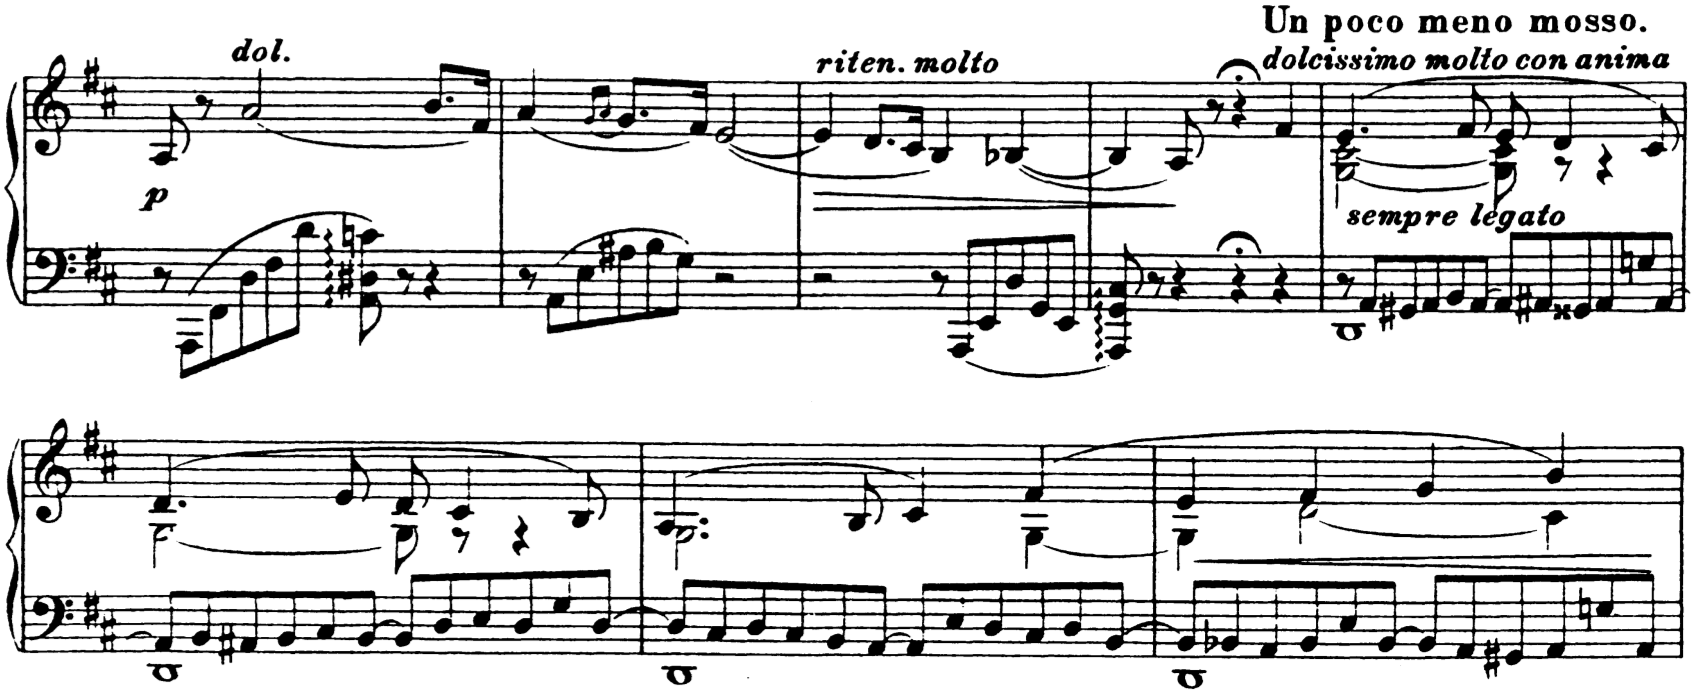
\includegraphics[width=12.5cm, keepaspectratio]{sonate-theme-3.png}
      &
      
\includegraphics[width=3cm, keepaspectratio]{op1-qr.png}
    \end{tabular}
  \end{bigcenter}
  \caption{\label{sonate-theme-1}Sonate en fa m Op.25, thème \no 3.}
\end{figure}

\begin{figure}[!p]
  \begin{bigcenter}
    \begin{tabular}{lr}
      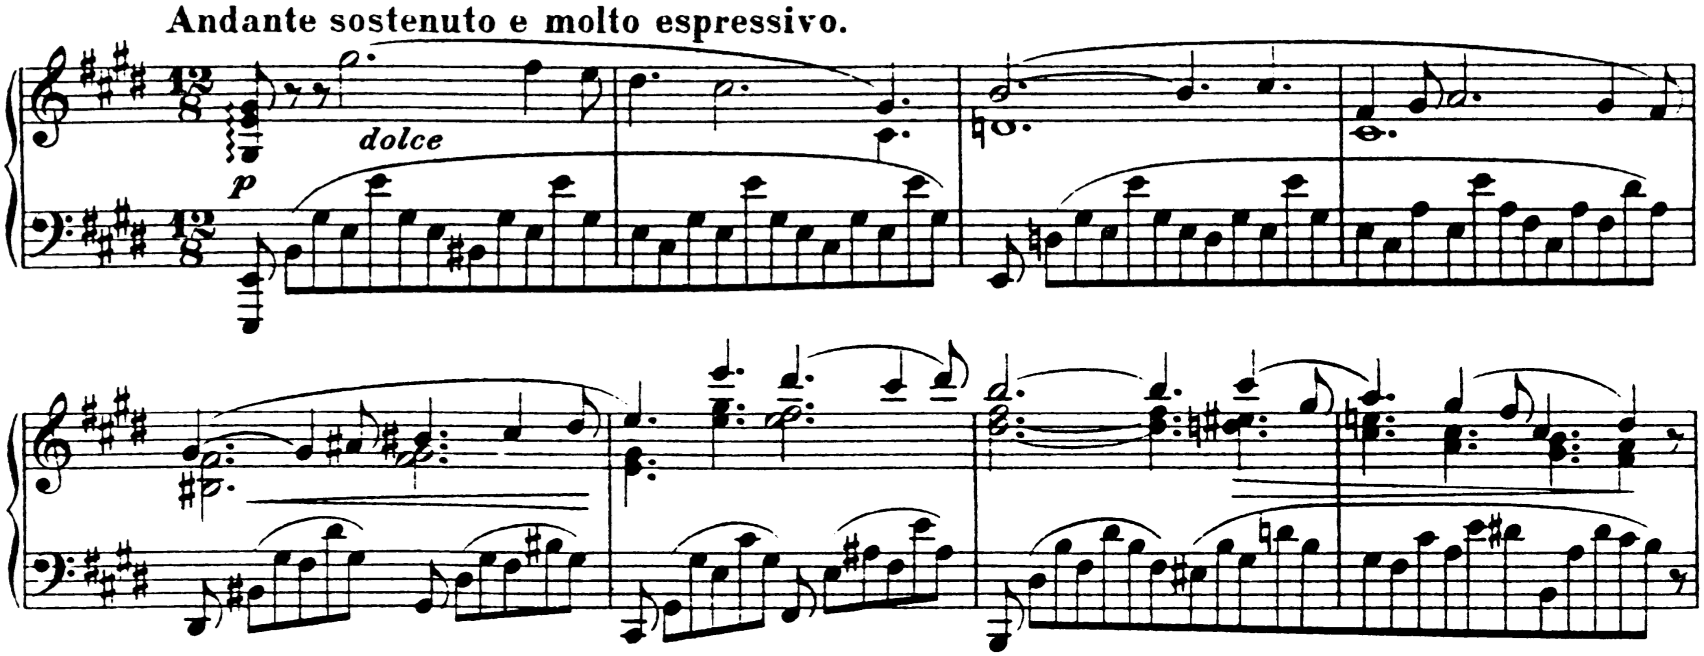
\includegraphics[width=12.5cm, keepaspectratio]{sonate-theme-4.png}
      &
      
\includegraphics[width=3cm, keepaspectratio]{op1-qr.png}
    \end{tabular}
  \end{bigcenter}
  \caption{\label{sonate-theme-1}Sonate en fa m Op.25, thème \no 4.}
\end{figure}

\begin{figure}[!p]
  \begin{bigcenter}
    \begin{tabular}{lr}
      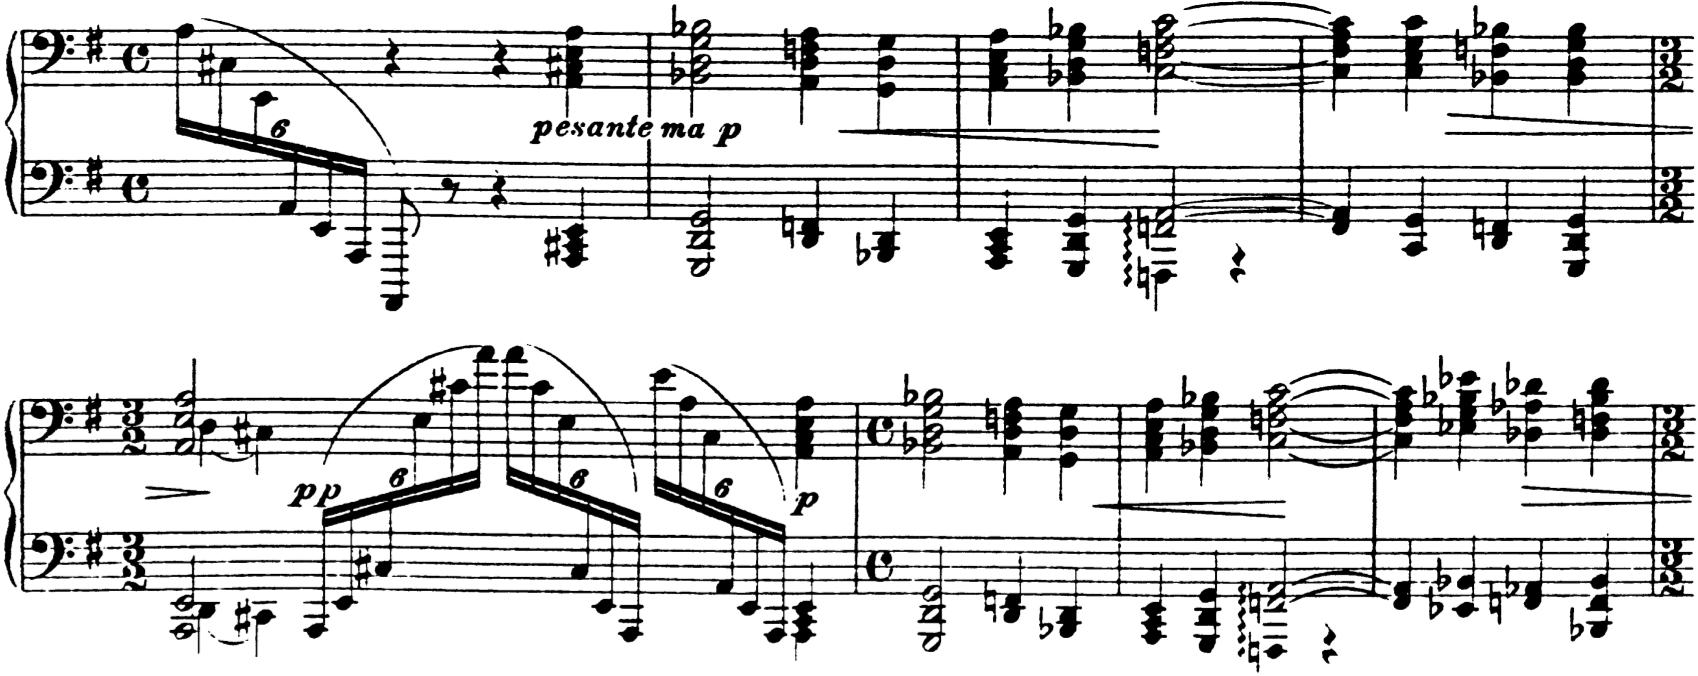
\includegraphics[width=12.5cm, keepaspectratio]{sonate-theme-5.png}
      &
      
\includegraphics[width=3cm, keepaspectratio]{op1-qr.png}
    \end{tabular}
  \end{bigcenter}
  \caption{\label{sonate-theme-1}Sonate en fa m Op.25, thème \no 5.}
\end{figure}

\begin{figure}[!ht]
  \begin{bigcenter}
    \begin{tabular}{lr}
      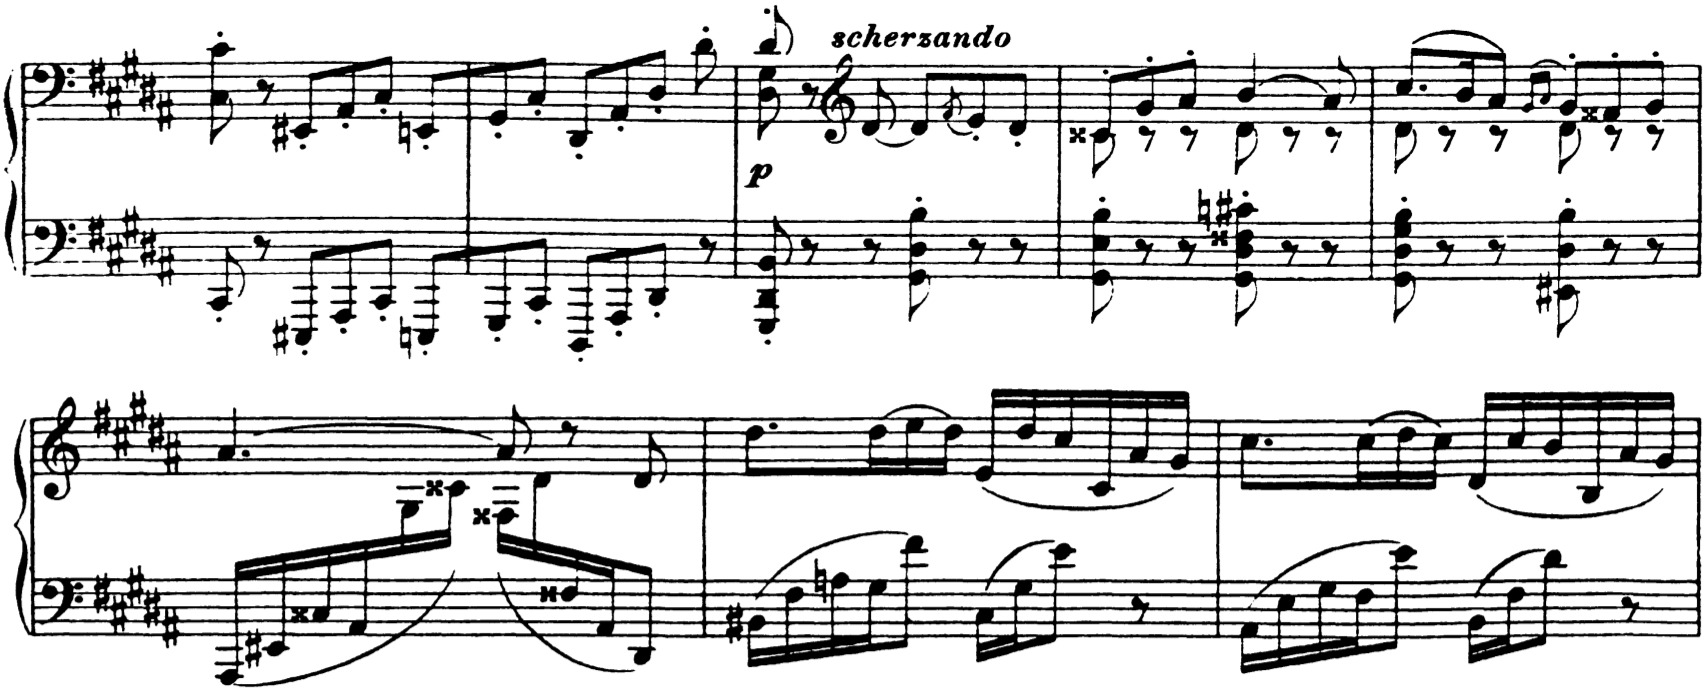
\includegraphics[width=12.5cm, keepaspectratio]{sonate-theme-6.png}
      &
      
\includegraphics[width=3cm, keepaspectratio]{op1-qr.png}
    \end{tabular}
  \end{bigcenter}
  \caption{\label{sonate-theme-1}Sonate en fa m Op.25, thème \no 6.}
\end{figure}

%%%%%%%%%%%%%%%%%%%%%%%%%%%%%%%%%%%%%%%%%%%%%%%%%%%%%%%%%%%%%%%%%%%%%%%%%%%%%
